\documentclass{report}
\usepackage[francais]{babel}
\usepackage{graphicx}
\usepackage{lmodern}
\usepackage{minted}


\begin{document}
\begin{titlepage}
  \centering
  {\scshape Institut Saint Jean Berchmans - Sainte Marie\par\vspace{0.2cm} Section informatique\par \vspace{0.2cm}}
  \vspace{1cm}
  
\includegraphics[width=0.25\textwidth]{img/image2}\par\vspace{1cm}
  {\scshape \LARGE Programmation \par}
  \vspace{0.2cm}
	{\scshape \Large The Shell Adventure\par}
  \vspace{3cm}
  {\Large\itshape Travail de fin d'étude \par réalisé par \par Jordan Dalcq \par}
  \vfill
  \scshape Année académique 2018 - 2019
  \title{The Shell Adventure}
  \author{Jordan Dalcq}
  \date{2018 - 2019}
\end{titlepage}

\pagestyle{headings}
\tableofcontents
\part*{Remerciments}

Je tiens tout d'abord à remercier mon grand père Yvan, qui m'a introduit au monde de l'informatique dés mon plus jeune âge, et de m'avoir montré aussi les joies de Linux dés mes 7 ans.
\newline
\par Je remercie mes parents Fabienne et Marc pour avoir investis en moi afin de me permettre de continuer sur ma voie vers un métier qui me pasionne.
\newline
\par Je remercie Alex Roşca, d'avoir été mon premier amis, dans cette grande aventure, merci de m'avoir permis de découvrire la programmation
\newline
\par Je remercie Monsieur David Carrera pour avoir été le seule professeur qui a été capable à me poussé au meillieur dans ma passion.
\newline
\par Je tiens aussi à remercier toutes les personne que j'ai rencontré à l'Institut Saint Jean Berchmans, pour m'avoir influencé dans ce projet d'une manière ou d'une autre.

\part{Introductions}

\section*{Contexte}
Durant quelques années j’ai été mentor au Coderdojo de Liège durant 2 ans. J’animais un atelier Python / Linux auprès de jeunes âgés entre 14 et 18 ans. Le problème lors de l’apprentissage était qu’ils ne savaient pas quelle commande / fonction utiliser dans un cas précis. Dans ce projet, j’ai décidé de me focaliser sur le terminal bash et de présenter un outil d’ apprentissage basé sur le visuel.
\chapter{Présentation}
\section{Fonctionnement}
L’idée de base est assez simple, il faut taper des commandes pour interagir avec le monde qui nous entoure.
\newline
\newline
Comme par exemple:

\begin {itemize}
  \item cd  : Pour se déplacer d’une pièce à une autre
  touch : Pour créer un objet ou bien faire apparaître une personne
  \item cp : Pour cloner un objet ou personnage
  \item mv : Pour déplacer un objet ou personnage
  \item cat : Pour connaître le contenu d’un objet ou alors l'identité d’un personnage
  \item rm : Pour jeter un objet ou “éliminer” un personnage
  \item tree : Scanner à rayon X pour voir à travers les murs
\end {itemize}

A cause du temps assez limité, j'ai implimenté un langage de programmation afin de laisser une liberté de choisir le pouvoir de chaque commande à l'utilisateur

\section{Élement}
Énumérez et décrivez, dans l’ordre et en français, les différentes parties de votre application. Il s’agit de présenter les différents éléments (ainsi que leurs caractéristiques) qui sont amenés à interagir au sein de votre programme.

\newpage

\begin{figure}[hb!]
  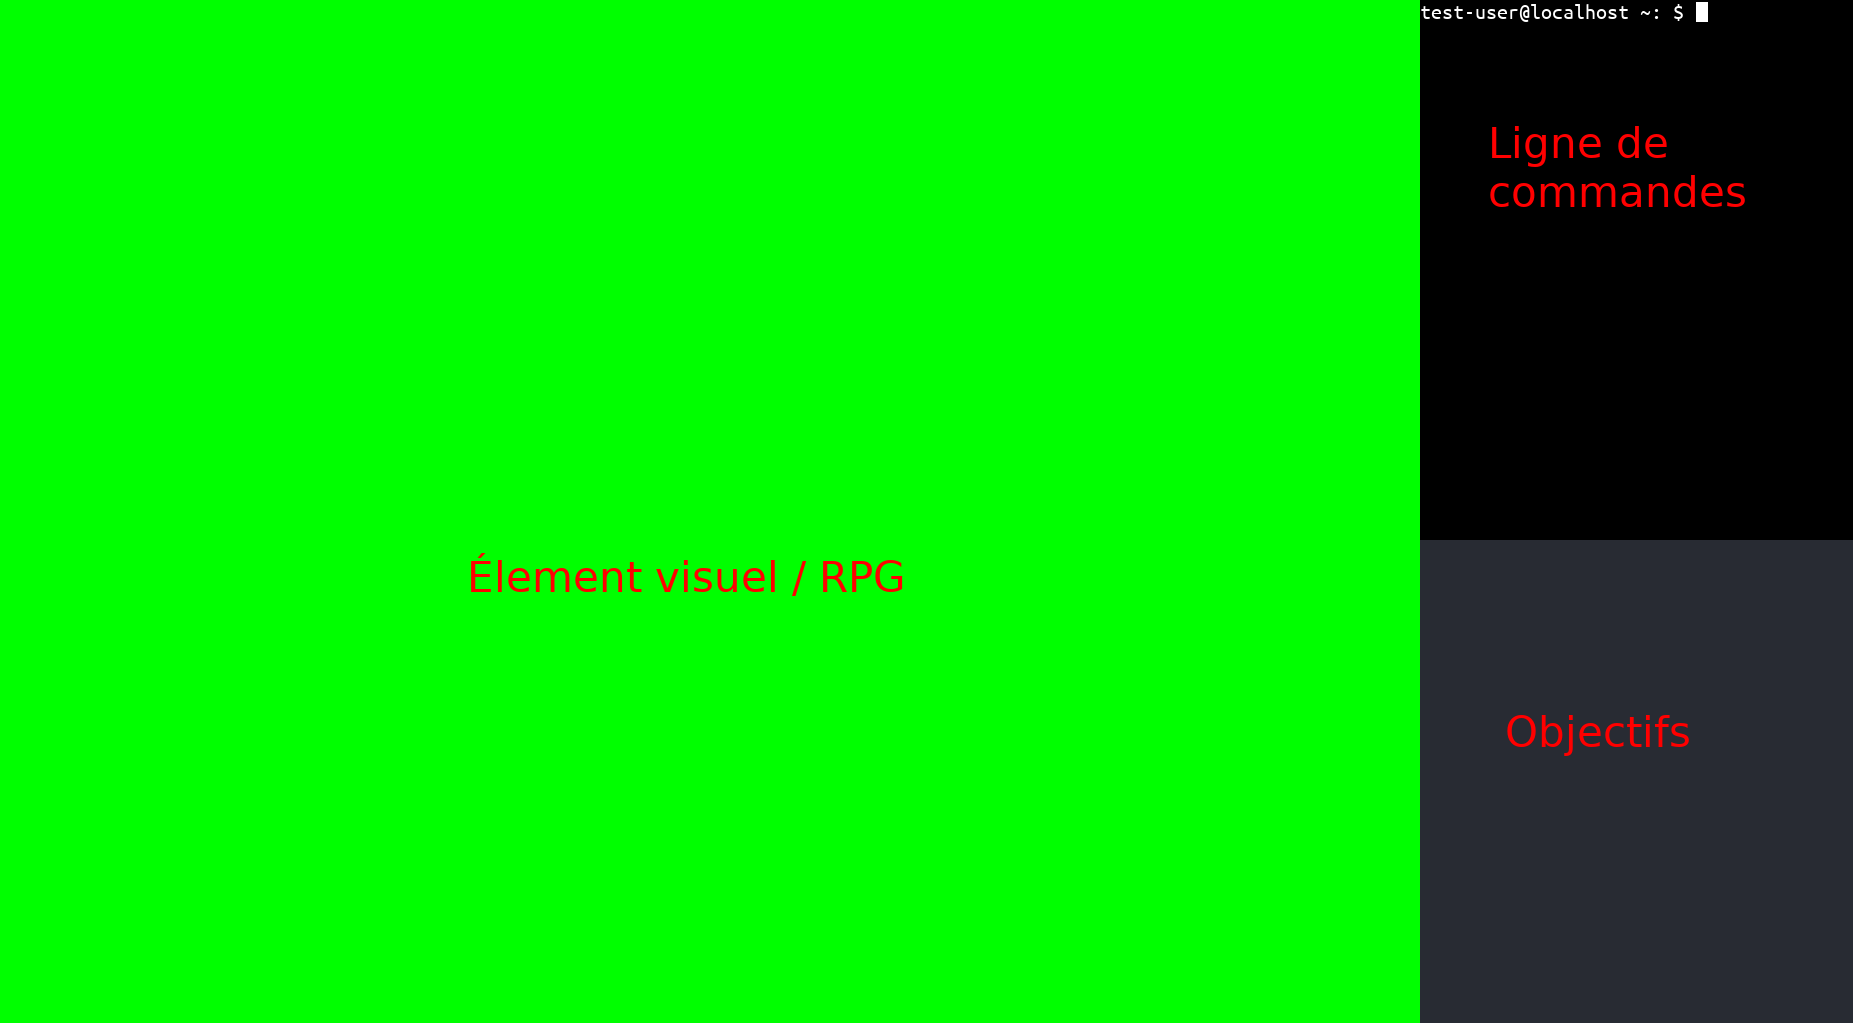
\includegraphics[width=\linewidth]{img/image1}
  \caption{Capture d'écran de la disposition par défault}
  \label{fig:screen1}
\end{figure}
\section {Interface utilisateur}
Par défaut, l’interface du jeu se présente comme représenté sur la figure \ref{fig:screen1}
\begin{description}
  \item [Élément visuel / RPG:] Là où seront dessinés les personnages et objet (armoir, chaise, garage, maison …)
  \item [Ligne de commandes:] Permet d’introduire des lignes de commande SH, qui seront interprétés par la suite.
  \item [Objectifs:] Permet d’afficher les tâches que le joueur doit effectuer
\end{description}
\par Il est aussi important de noter que chaque scripts est libre de changer cette disposition comme bon
l'entend


\chapter{Analyse}
\section{Classes}
\subsection{game.mechanics.term.Term}
La classe \emph{Term} permet de créer des surfaces d'interaction tel que ligne de commande et entrée standard pour l’utilisateur, une fois initialisé elle charge la police de caractères monospace (en 22 pixels car c’est beaucoup plus lisible et agréable à utiliser), ensuite elle crée un dossier \emph{.shelladv} dans le dossier personnel de l’utilisateur (Exemple: \emph{/home/dalcjor/.shelladv} )
\subsection*{Attributs}
\begin{itemize}
  \item \mintinline{python}{surface : pygame.Surface}		$\rightarrow$ Surface principale du terminal
  \item \mintinline{python}{mono : pygame.font.Font}		$\rightarrow$ Police de caractère monospace
  \item \mintinline{python}{visualLine : List[str]}		$\rightarrow$ Lignes visibles sur la surface du terminal
  \item \mintinline{python}{lineRect : pygame.Rect}		$\rightarrow$ Rectangle de l’entrée utilisateur
  \item \mintinline{python}{blinkRect : pygame.Rect}		$\rightarrow$ Rectangle avec le rectangle clignotant
  \item \mintinline{python}{fontSurface : pygame.Rect}		$\rightarrow$ Rectangle avec les lignes précédentes
  \item \mintinline{python}{inInput : bool}			$\rightarrow$ Permet de savoir si l’utilisateur est en train d'entrer du texte
  \item \mintinline{python}{promptVisual: bool}			$\rightarrow$ Permet de savoir si le terminal doit afficher le prompt
  \item \mintinline{python}{bash: bool}				$\rightarrow$ Permet de savoir si le terminal doit exécuter les commandes entrées ou pas
  \item \mintinline{python}{currentTyping : str}		$\rightarrow$ Stock l’entrée utilisateur
  \item \mintinline{python}{blinkX : int}			$\rightarrow$ Position x du rectangle clignotant à côté du prompt
  \item \mintinline{python}{custom : str}			$\rightarrow$ Stock les prompts customisés
  \item \mintinline{python}{history : mechanics.term.History}	$\rightarrow$ Stock les prompts customisés
  \item \mintinline{python}{env : Dict[str, str]}		$\rightarrow$ Variables d'environnements semblables à celles présentes dans les systèmes UNIX
  \item \mintinline{python}{prompt: str}		$\rightarrow$ Permet de prendre connaissance du nom d’utilisateur, nom de la machine et le CWD (Current Work Directory)
  \item \mintinline{python}{tick: float}		$\rightarrow$ Heure actuel pour permettre de réguler la vitesse du blink (le rectangle à côté du prompt)
\end{itemize}

\subsection*{Méthodes}
\begin{itemize}
  \item \mintinline{python}{resize(size: Tuple[int, int])}		$\rightarrow$ Change la taille de la surface du terminal
  \item \mintinline{python}{disable_prompt()}		$\rightarrow$  cache le prompt
  \item \mintinline{python}{enable_prompt()}		$\rightarrow$ Ré-affiche le prompt
  \item \mintinline{python}{isprompt_enabled() : bool}		$\rightarrow$ Retourne \mintinline{python}{True} si le prompt est affiché
  \item \mintinline{python}{disable_bash()}		$\rightarrow$ Désactive l'exécution des entrées
  \item \mintinline{python}{enable_bash()}		$\rightarrow$ Réactive l'exécution des entrées
  \item \mintinline{python}{getInput()}		$\rightarrow$ Active l’entrée utilisateur
  \item \mintinline{python}{removeLine()}		$\rightarrow$ Supprime la dernière ligne affichée dans le terminal
  \item \mintinline{python}{set_custom_prompt(string: str)}		$\rightarrow$ Permet de mettre un prompt customisé
  \item \mintinline{python}{add_to_display(output: str)}		$\rightarrow$ Permet d’ajouter une ligne à l’attributs \mintinline{python}{visualLine}, qui servira ensuite pour l’affichage
  \item \mintinline{python}{clear()} $\rightarrow$ Permet d’effacer les lignes affichées à l’écran
  \item \mintinline{python}{get_env(): Dict[str, str]}		$\rightarrow$ Retourne les variables d'environnements
  \item \mintinline{python}{draw()}	$\rightarrow$ Permet de dessiner les lignes de commandes entrées par l’utilisateur
  \item \mintinline{python}{drawBlink()}		$\rightarrow$ Dessine le rectangle qui clignote à côté du prompt
  \item \mintinline{python}{keydown()}		$\rightarrow$ Méthode de traitement des touches pressées, pour ensuite les affichéer dans la console
  \item \mintinline{python}{update()}		$\rightarrow$  Méthode qui gère le curseur et appelle la méthode \mintinline{python}{draw}
  \item \mintinline{python}{get_surface(): pygame.Surface()}		$\rightarrow$ Actualise et retourne la surface du terminal
\end{itemize}
\newpage

\subsection{game.mechanics.term.History}
Comme dans tout bon shell, il y a un gestionnaire d’historique, cela permet de rechercher des commandes déjà tapées.
Les historiques sont sauvegardé de façon à ce que l'utilisateur puisse retrouver ces commandes dans le jeu.

\subsection*{Attributs}

\begin{itemize}
  \item \mintinline{python}{home: str}	$\rightarrow$ Chemin vers le dossier utilisateur
  \item \mintinline{python}{hist: file}		$\rightarrow$ Lien en lecture vers le fichier d’historique (\mintinline{bash}{\$HOME/.bash_history}) % To remove
\end{itemize}

\subsection*{Méthodes}
\begin{itemize}
\item \mintinline{python}{__getitem__(index: int) : str}	$\rightarrow$ retourne une ligne spécifique de l’historique
\item \mintinline{python}{append(line: str)}	$\rightarrow$  ajoute une ligne à l’historique
\item \mintinline{python}{openFile()}	$\rightarrow$ Ouvre le fichier d’historique
\item \mintinline{python}{get_size() : int}	$\rightarrow$ Retourne le nombre de commande présent dans l'historique
\item \mintinline{python}{get_previous() : str}	$\rightarrow$ Retourne la command qui a été précedemment introduite
\item \mintinline{python}{get_next()}	$\rightarrow$ Retourne la commande qui suis

\end{itemize}

\newpage

\subsection{game.mechanics.rpg.Rpg.Rpg}
La classe \mintinline{python}{Rpg} permet d’afficher les éléments visuels.

\subsection*{Attributs}
\begin{itemize}
  \item \mintinline{python}{sprites: Dict[str, game.mechanics.rpg.sprite.Sprite]}	$\rightarrow$ Dictionnaire qui lie un sprite à un nom (Le nom étant une variable du Adventure Script), ce dictionnaire contient tous les sprites à afficher à l’écran
  \item \mintinline{python}{surface: pygame.Surface}	$\rightarrow$ Surface du Rpg
\end{itemize}

\subsection*{Métohdes}
\begin{itemize}
  \item \mintinline{python}{add_to_surface(name: str, sprite: game.mechanics.rpg.sprite.Sprite)}	$\rightarrow$ Permet d’ajouter un sprite à l’écran
  \item \mintinline{python}{update()}	$\rightarrow$  Actualise la surface et applique les sprites à la surface
  \item \mintinline{python}{resize(size: Tuple[int, int])}	$\rightarrow$ Change la taille de la surface
\end{itemize}
\newpage

\subsection {game.mechanics.rpg.sprite.Sprite}
Cette classe permet de gérer les spritesheet automatiquement, grâce au \emph{Adventure Script} (voir autre dossier pour syntaxe), il est possible de gérer des spritesheet avec 4 actions dans cette ordre précis: Pars vers le haut, pars à Droite, pars à Gauche,  pars vers le bas. Le premier sprite doit être celui par défaut (au repos). Par contre vous pouvez mettre autant de frames à une action que vous voulez. Toutes les configurations nécessaires sont faites via \emph{Adventure Script}

\begin{figure}[hb!]
  \centering
  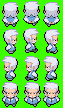
\includegraphics[width=3cm]{img/image3}
  \caption{Exemple de spritesheet compatible}
  \label{fig:spritesheet}
\end{figure}

\subsection*{Attributs}
\begin{itemize}
  \item \mintinline{python}{size: Tuple[int, int]}		$\rightarrow$ Taille d’une frame du sprite
  \item \mintinline{python}{finalSize: Tuple[int, int]}		$\rightarrow$ Taille finale d’une frame (car elles sont souvent trop petites)
  \item \mintinline{python}{index: Tuple[int, int]}		$\rightarrow$ Position de la frame actuelle
  \item \mintinline{python}{spriteSurface: pygame.Surface}		$\rightarrow$ Surface dédiée à une frame
  \item \mintinline{python}{spriteSheet: pygame.Surface}		$\rightarrow$ Surface qui contient toute la spritesheet au complet
  \end{itemize}
\subsection*{Méthodes}
\begin{itemize}
  \item \mintinline{python}{get_pos() : Tuple[int, int] }		$\rightarrow$ Retourne la position du sprite sur la Surface dédié au RPG
  \item \mintinline{python}{get_surface(): pygame.Surface}		$\rightarrow$ Applique une frame à l’attribut \item \mintinline{python}{spriteSurface} et retourne la surface
  \item \mintinline{python}{reset(index: int)}		$\rightarrow$ Met le sprite à une position repos en fonction de sa direction, s’il est à sa dernière frame ou s’il change de direction
  \item \mintinline{python}{move(self, way: int)}		$\rightarrow$ Fait passer le sprite à sa frame suivante
  \item \mintinline{python}{stop(way: int)}		$\rightarrow$ Met le sprite en repos, car il a fini de se déplacer
\end{itemize}
\newpage
\begin{figure}[hb!]
  \centering
  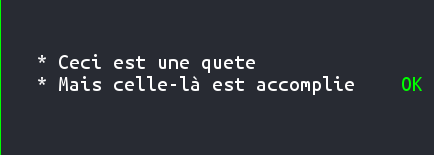
\includegraphics[width=10cm]{img/image4}
  \caption{Exemple de quêtes}
  \label{fig:spritesheet}
\end{figure}
\subsection{game.mechanics.quest.Quest.Quest}
Cette classe permet de gérer les quêtes grâce au langage implémenté dans le jeu (voir autre dossier pour syntaxe). Il est important de noter que le jeu est limité à 18 quêtes à la fois.

\end{document}
